\section{Sviluppi futuri}
Non tutti i casi d'uso definiti sono stati implementati. Di seguito è riportata una tabella riassuntiva di quali casi d'uso sono stati implementati e quali no.

\begin{table}[h!]
	\centering
	\begin{tabular}{|c|c|c|}
		\hline
		\textbf{Codice} & \textbf{Caso d'uso} & \textbf{Implementato} \\ \hline
		\multicolumn{3}{|c|}{Alta Priorità} \\ \hline
		\textbf{UC1} & Login & Sì\\ \hline
		\textbf{UC2} & Logout & Sì \\ \hline
		\textbf{UC3} & Visualizzazione informazioni account & Sì \\ \hline
		\textbf{UC4} & Visualizzazione informazioni squadra & Sì \\ \hline
		\textbf{UC15} & Inserimento utente & Sì \\ \hline
		\textbf{UC16} & Cancellazione utente & Sì\\ \hline
		\textbf{UC17} & Gestione squadre (creazione) & Sì \\ \hline
		\textbf{UC18} & Visualizzazione informazioni zona & Sì \\ \hline
		\multicolumn{3}{|c|}{Media Priorità} \\ \hline
		\textbf{UC6} & Segnalazione operatività & Sì\\ \hline
		\textbf{UC7} & Visualizzazione intervento di emergenza & No \\ \hline
		\textbf{UC8} & Visualizzazione intervento programmato & No \\ \hline
		\textbf{UC9} & Inserimento informazioni intervento & No \\ \hline
		\textbf{UC11} & Gestione intervento di emergenza & No \\ \hline
		\textbf{UC12} & Gestione intervento programmato & No \\ \hline
		\textbf{UC13} & Gestione report intervento di emergenza & No \\ \hline
		\textbf{UC14} & Gestione report intervento programmato & No \\ \hline
		\textbf{UC20} & Gestione informazioni relative alla zona & No \\ \hline
		\multicolumn{3}{|c|}{Bassa Priorità} \\ \hline
		\textbf{UC5} & Gestione reperibilità & No\\ \hline
		\textbf{UC10} & Visualizzazione posizione real-time & Sì\\ \hline
		\textbf{UC19} & Notifiche allarmi zona & No\\ \hline
	\end{tabular}
	\caption{\label{tab:table-name}Casi d'uso implementati e mancanti.}
\end{table}


\section{Approfondimento - Qt}
Qt è un framework per lo sviluppo di applicazioni cross-platform: con un unico codice è possibile creare applicazioni in grado di girare su diversi sistemi operativi, come Windows, MacOS, Android e iOS. Il linguaggio su cui si basa è il C++ ma è possibile utilizzare anche altri linguaggi, come Python e Java. La potenzialità del framework Qt è la sua architettura modulare con un elevato livello di astrazione rispetto la piattaforma sottostante. Il modulo principale, \textit{QtCore}, include l'implementazione di svariate strutture dati, inclusi tipi generici e classi apposite per la manipolazione delle stringhe di testo. Per la creazione di interfacce grafiche, uno dei componenti principali è il \textit{Qt Widget}, che viene utilizzato principalmente per lo sviluppo in ambito Desktop. Per applicazioni embedded, invece, viene utilizzato il modulo \textit{QtQuick} che garantisce una maggiore separazione tra le entità coinvolte nell'implementazione dell'interfaccia grafica e quelle che riguardano la \textit{business logic} dell'applicazione. 
\\
In questo progetto è stato utilizzato il C++ come linguaggio di programmazione per la \textit{business logic}, mentre per la parte grafica è stato utilizzato il modulo \textit{QtQuick} con il \textit{QML} (\textit{Qt Modelling Language}), un linguaggio dichiarativo basato su JavaScript. 

\begin{figure}[h!]
	\centering
	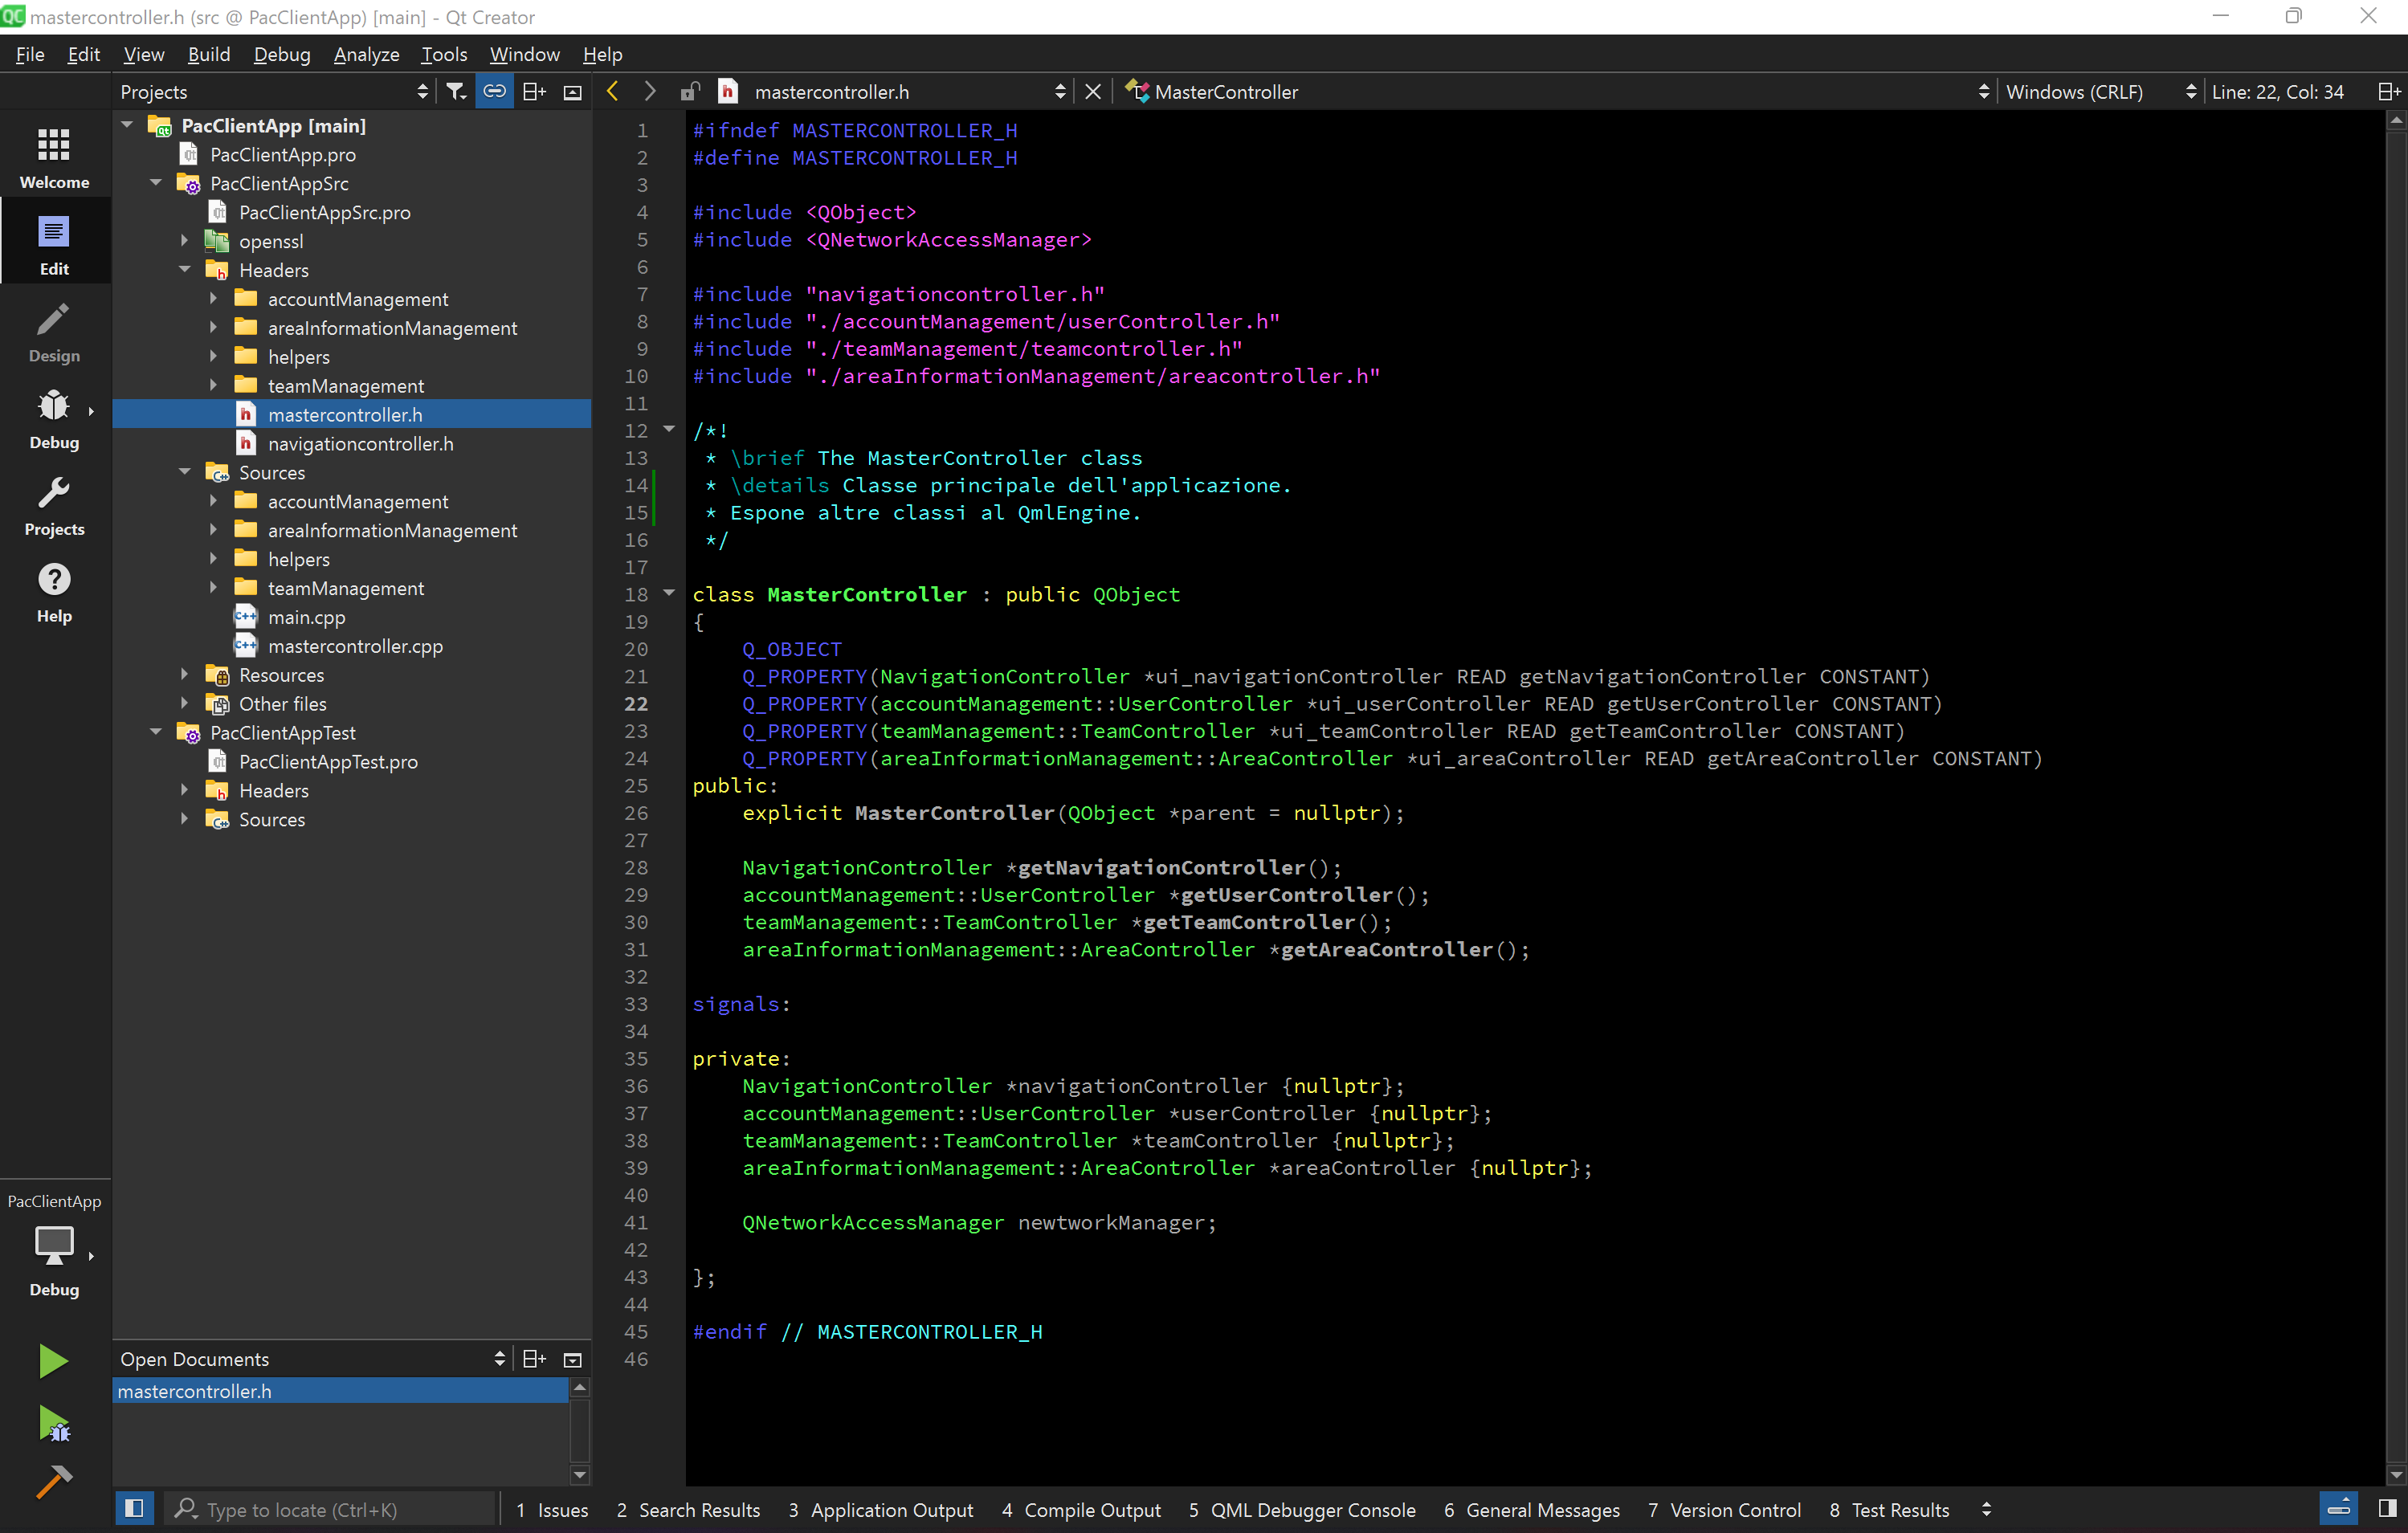
\includegraphics[width=0.8\linewidth]{./Conclusione/ImageFiles/Qt Framework}
	\caption{Schermata dell'IDE \textit{Qt Creator} con il progetto aperto.}
	\label{fig:qtFramework}
\end{figure}

Il progetto è stato strutturato come mostrato in figura \ref{fig:StrutturaProg}. È stato creato un progetto principale, nominato \texttt{PacClientApp}, che contiene due sotto progetti: \texttt{PacClientAppSrc} è il progetto che contiene i sorgenti relativi all'applicazione, mentre \texttt{PacClientAppTest} è il progetto che contiene i file per eseguire i test automatici grazie al modulo \textit{QtTest}. All'interno di \texttt{PacClientAppSrc}, sono state create delle sotto cartelle per la gestione dei \textit{namespace} in C++, che sono l'equivalente dei \textit{package} in Java. Le sottocartelle create sono le stesse inserite lato server, e riflettono l'architettura dell'applicazione. L'unico \textit{namespace} estraneo è l\texttt{helpers}, che contiene alcune classi con delle funzioni di supporto che vengono utilizzate in diversi punti dell'applicazione.  
\\
All'interno dei \textit{namespace} è stata creata una componente \textit{controller} che si occupa di effettuare le richieste tramite API REST al server e di gestire le risposte.


\begin{figure}[h!]
	\centering
	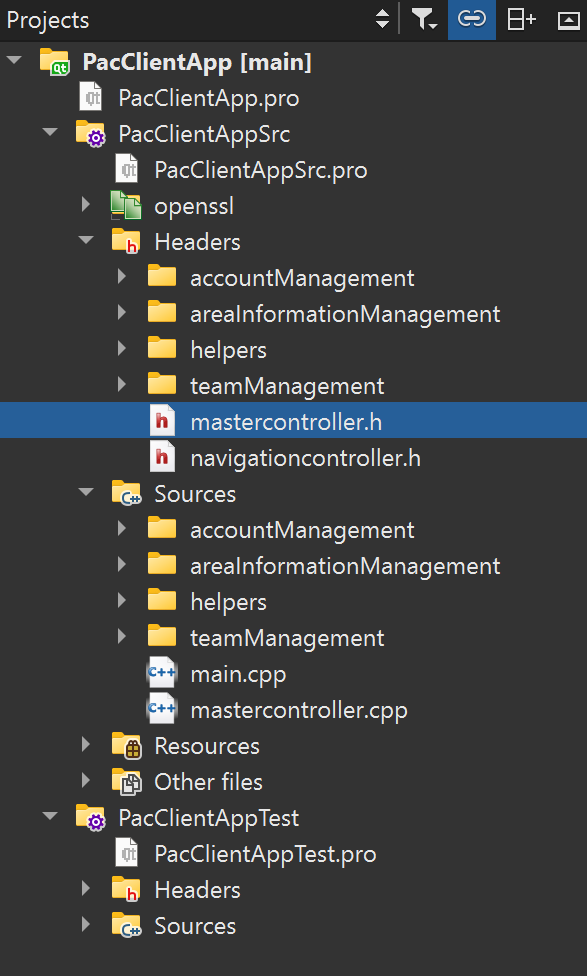
\includegraphics[width=0.4\linewidth]{./Conclusione/ImageFiles/strutturaProgettoQt}
	\caption{Schermata dell'IDE \textit{Qt Creator} con il progetto aperto.}
	\label{fig:StrutturaProg}
\end{figure}